\chapter{Praktisches Beispiel}
\label{chap:praktischesBeispiel}
\section{Zielsetzung}
\label{sec:zielsetzung}
\printsubchapterauthor{\authorMarco}
Zur Darstellung eines Netzes, welches mithilfe von TensorFlow erstellt und trainiert wurde, soll im Zuge dieser Arbeit einen Demonstrator entwickelt werden. Das gewählte Beispiel ist die Erkennung von handgeschriebenen Ziffern. Dabei sollen vor allem die Effekte unterschiedlicher Lernraten auf die Richtigkeit der Vorhersagen untersucht werden.

Weiterhin wird auf die Nutzung des Berechnungsgraphen eingegangen und aufgezeigt, wie dieser im Demonstrator funktioniert. Dies betrifft ebenfalls die eingesetzten Operatoren und die Transformation der Tensoren.

Im Anschluss wird auf Probleme eingegangen, welche beim Erstellen und Trainieren des Netzes aufgetreten sind.

\section{Datensätze}
\label{sec:datensaetze}
\printsubchapterauthor{\authorMarco}
Der Datensatz, der zum Trainieren und Überprüfen des Netzes genutzt wurde, ist der MNIST Datensatz. Dieser Datensatz wurde von dem National Institute of Standards and Technology angefertigt und besteht aus 60.000 Trainingsziffern und 10.000 Testziffern. Alle Zahlen sind handgeschrieben und auf eine Größe von 28x28 Pixeln verkleinert. Die einzelnen Ziffern weisen verschiedene Graustufen in ihrer Darstellung auf.

\section{Erstellen des Netzes}
\label{sec:erstellenDesNetzes}
\printsubchapterauthor{\authorNiklas}
Der Datensatz, der für das neuronale Netz genutzt wird besteht aus Bildern mit einer Größe von 28x28 Pixeln. Da dem neuronalen Netz jedes Pixel übergeben werden soll, muss zuerst die Länge des Eingangsarrays berechnet werden.
\begin{center} 28 * 28 = 784\end{center}
Das Eingangsarray besitzt eine Länge von 784 Einträgen. Daher muss die Eingabeschicht des neuronalen Netzes ebenfalls 784 Platzhalter besitzen, die diese Werte entgegennehmen. Da es sich bei den handgeschriebenen Zahlen nur um die Zahlen von 0 bis 9, also 10 Zahlen, handelt, benötigt das neuronale Netz eine Ausgangsschicht mit 10 Tensoren. Zur Anpassung der Gewichte wird im Training die Softmax-Regression oder auch logistische Regression verwendet. Der gesamte Datenflussgraph ist in der Abbildung \ref{fig:demonstratorGraph} zu sehen.
\pagebreak
\begin{center}
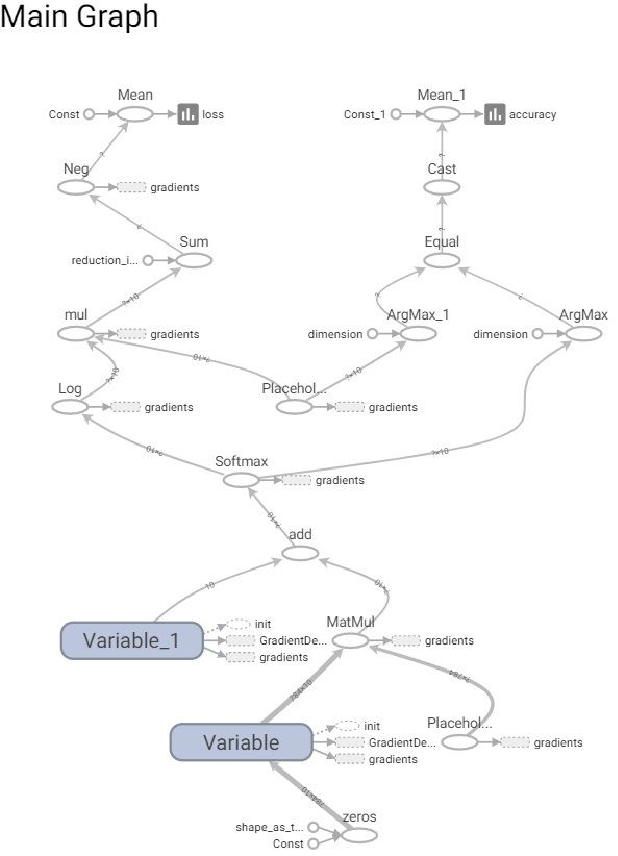
\includegraphics[width=.6\textwidth]{../abbildungen/DemonstratorGraph.pdf}
	\captionof{figure}{Datenflussgraph des Beispiels}
	\label{fig:demonstratorGraph}
\end{center} 
Nach dem Trainieren wird zu jeder Zahl ein Thumbnail angezeigt, das darstellt, welcher Pixelbereich ungefähr gesetzt sein muss, damit das neuronale Netz diese Zahl in dem Bild interpretiert. Der Code des gesamten neuronalen Netzes ist im Anhang \ref{sec:codeDemonstrator} zu finden.

\section{Auswertung}
\label{sec:auswertung}
\printsubchapterauthor{\authorMarco}
Das Netz wurde nach dem Erstellen mit verschiedenen Lernraten trainiert und validiert. Dabei wurden immer 20.000 der 60.000 Testbilder für eine Trainingssession genutzt. Die untersuchten Lernraten lagen zwischen 0,0001 und 1. Für Lernraten, die kleiner als 0,005 waren, lag die Richtigkeit der erkannten Zahlen bei unter 90\%. Lernraten zwischen 0,08 und 0,5 ergaben die besten Ergebnisse mit über 92\% Genauigkeit. Bei Lernraten, die über 0,5 hinausgingen, nahm die Genauigkeit wieder ab. Die beste Genauigkeit wurde bei einer Lernrate von 0,3 erzielt.

Faktoren, die diese Ergebnisse beeinflussen, sind allerdings nicht nur die Lernrate. Auch die Anzahl der genutzten Bilder in einer Trainingssession hat einen großen Einfluss auf das Ergebnis, da mehr Bilder zu einer besseren Genauigkeit führen. Weiterhin unterscheiden sich die Genauigkeiten ab einer Lernrate von 0,005 nur um wenige Prozentpunkte.

Die verschiedenen Gewichtungen bei unterschiedlichen Lernraten geben einen interessanten Einblick darauf, wie das neuronale Netz die Zahlen wahrnimmt.
\begin{center}
	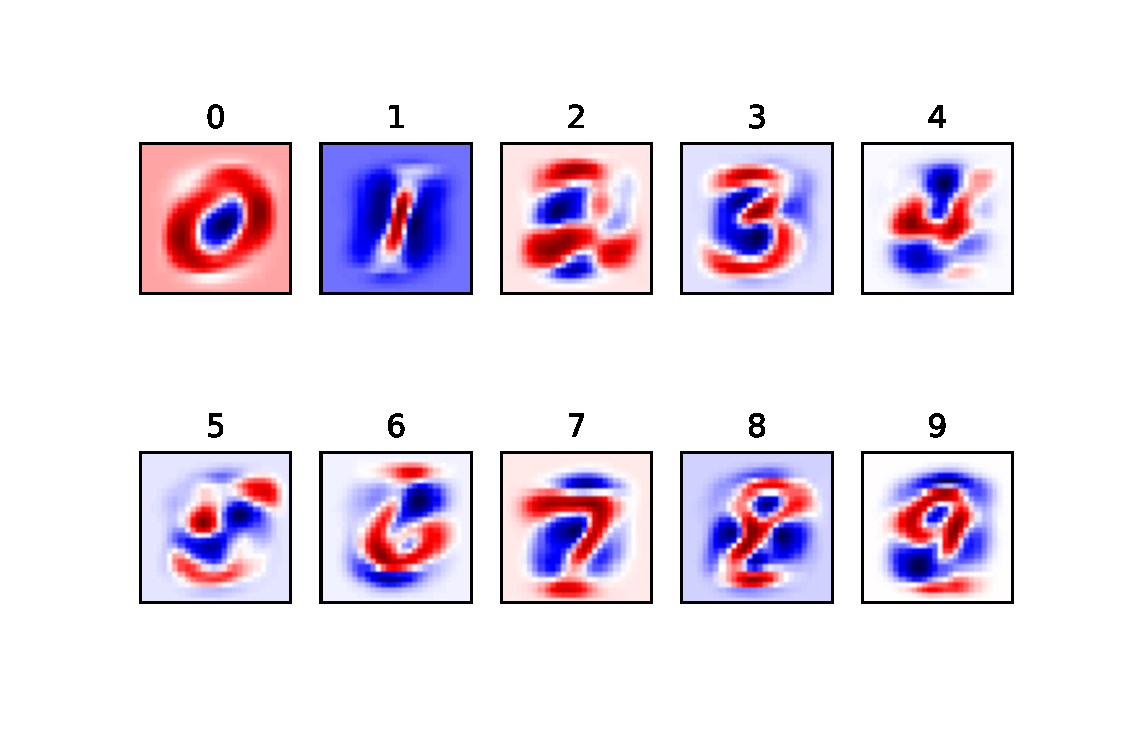
\includegraphics[width=.6\textwidth]{../abbildungen/weightPlot00001.pdf}
	\captionof{figure}{Gewichtungen bei einer Lernrate von 0.0001}
	\label{fig:gewichtung00001}
\end{center}

Wie in Abbildung \ref{fig:gewichtung00001} zu sehen ist, werden bei einer niedrigen Lernrate die Gewichtungen auf die einzelnen Werte so angepasst, dass die Ziffern in den Bildern für den Menschen klar erkenntlich sind. Allerdings ist dieses Vorgehen sehr langsam.

\begin{center}
	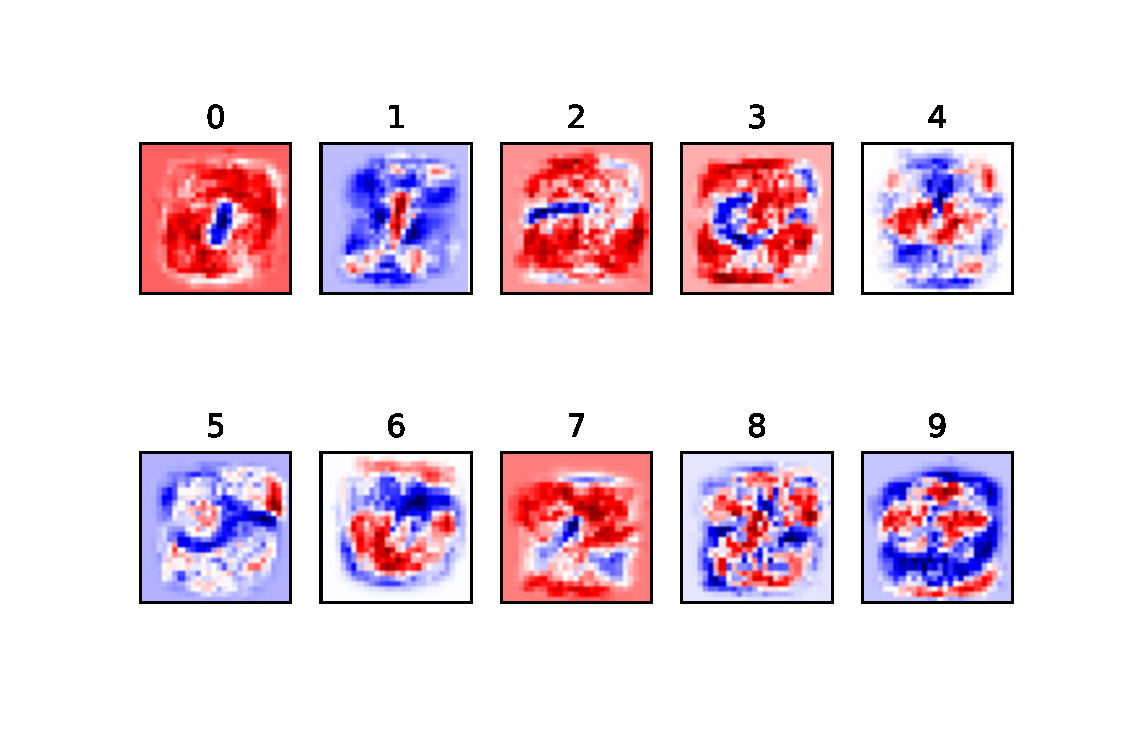
\includegraphics[width=.6\textwidth]{../abbildungen/weightPlot0008.pdf}
	\captionof{figure}{Gewichtungen bei einer Lernrate von 0.08}
	\label{fig:gewichtung0008}
\end{center}

In Abbildung \ref{fig:gewichtung0008} ist eine höhere Lernrate verwendet wurden. Dabei sind die einzelnen Ziffern nicht mehr für den Menschen erkennbar bzw. nur noch zu erraten. Dafür wurde mit dieser Variante eine höhere Genauigkeit erzielt. Generell gilt, je höher die Lernrate ausfällt, desto schlechter sind Ziffern erkennbar.

\section{Probleme}
\label{sec:probleme}
\printsubchapterauthor{\authorNiklas}
Bei der Erstellung des neuronalen Netzes selbst sind keine großen Problem aufgetreten. Die einzigen Probleme, die auftraten fanden bei der Installation statt. Die einfachste Variante der Installation ist über eine virtuelle Umgebung von Anaconda. In dieser virtuellen Umgebung kann TensorFlow installiert werden, ohne die Python-Installation des Rechners zu verändern. Auf einem Mac ist ein relativ neues Betriebssystem nötig, um TensorFlow nutzen zu können. Das Betriesbssystem \textit{El Capitan} reicht dafür nicht aus. Auf einem Ubuntu 18.04 Rechner müssen nach abgeschlossener Installation manche Bibliotheken einzeln installiert werden. Auf einem Windows-Computer werden alle nötigen Bibliotheken bei der Installation mit installiert und TensorFlow ist nach der Installation einsatzbereit.